\documentclass[aspectratio=169]{beamer}
\usepackage{../pomozno/prosojnice}

\begin{document}
\begin{frame}[fragile]
  \begin{center}
    \Huge\textbf \LaTeX
  \end{center}
\end{frame}

\begin{frame}
  \vspace{1em}
  \begin{center}
    {\Huge Donald E. Knuth}
    \bigskip

    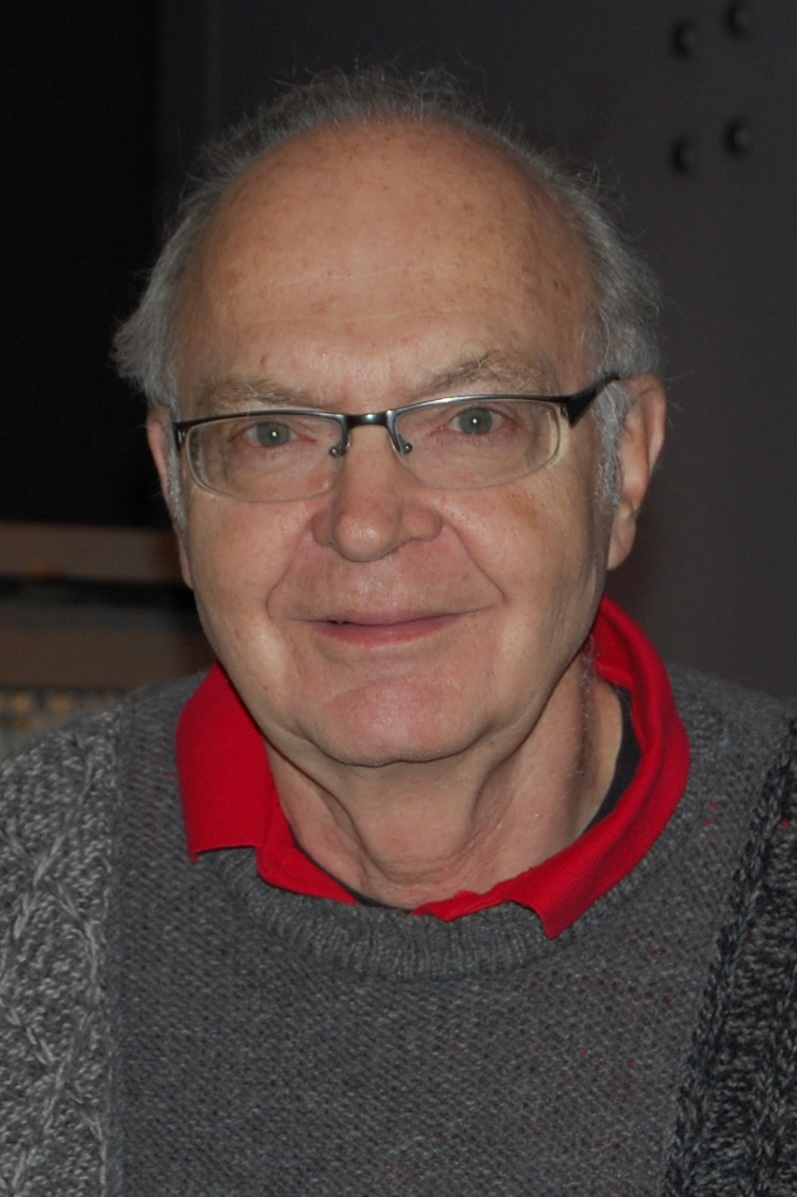
\includegraphics[height=0.65\textheight,keepaspectratio]{knuth.jpg}
    \smallskip

    dobitnik Turingove nagrade (1974)
  \end{center}
\end{frame}

\usebackgroundtemplate{%
  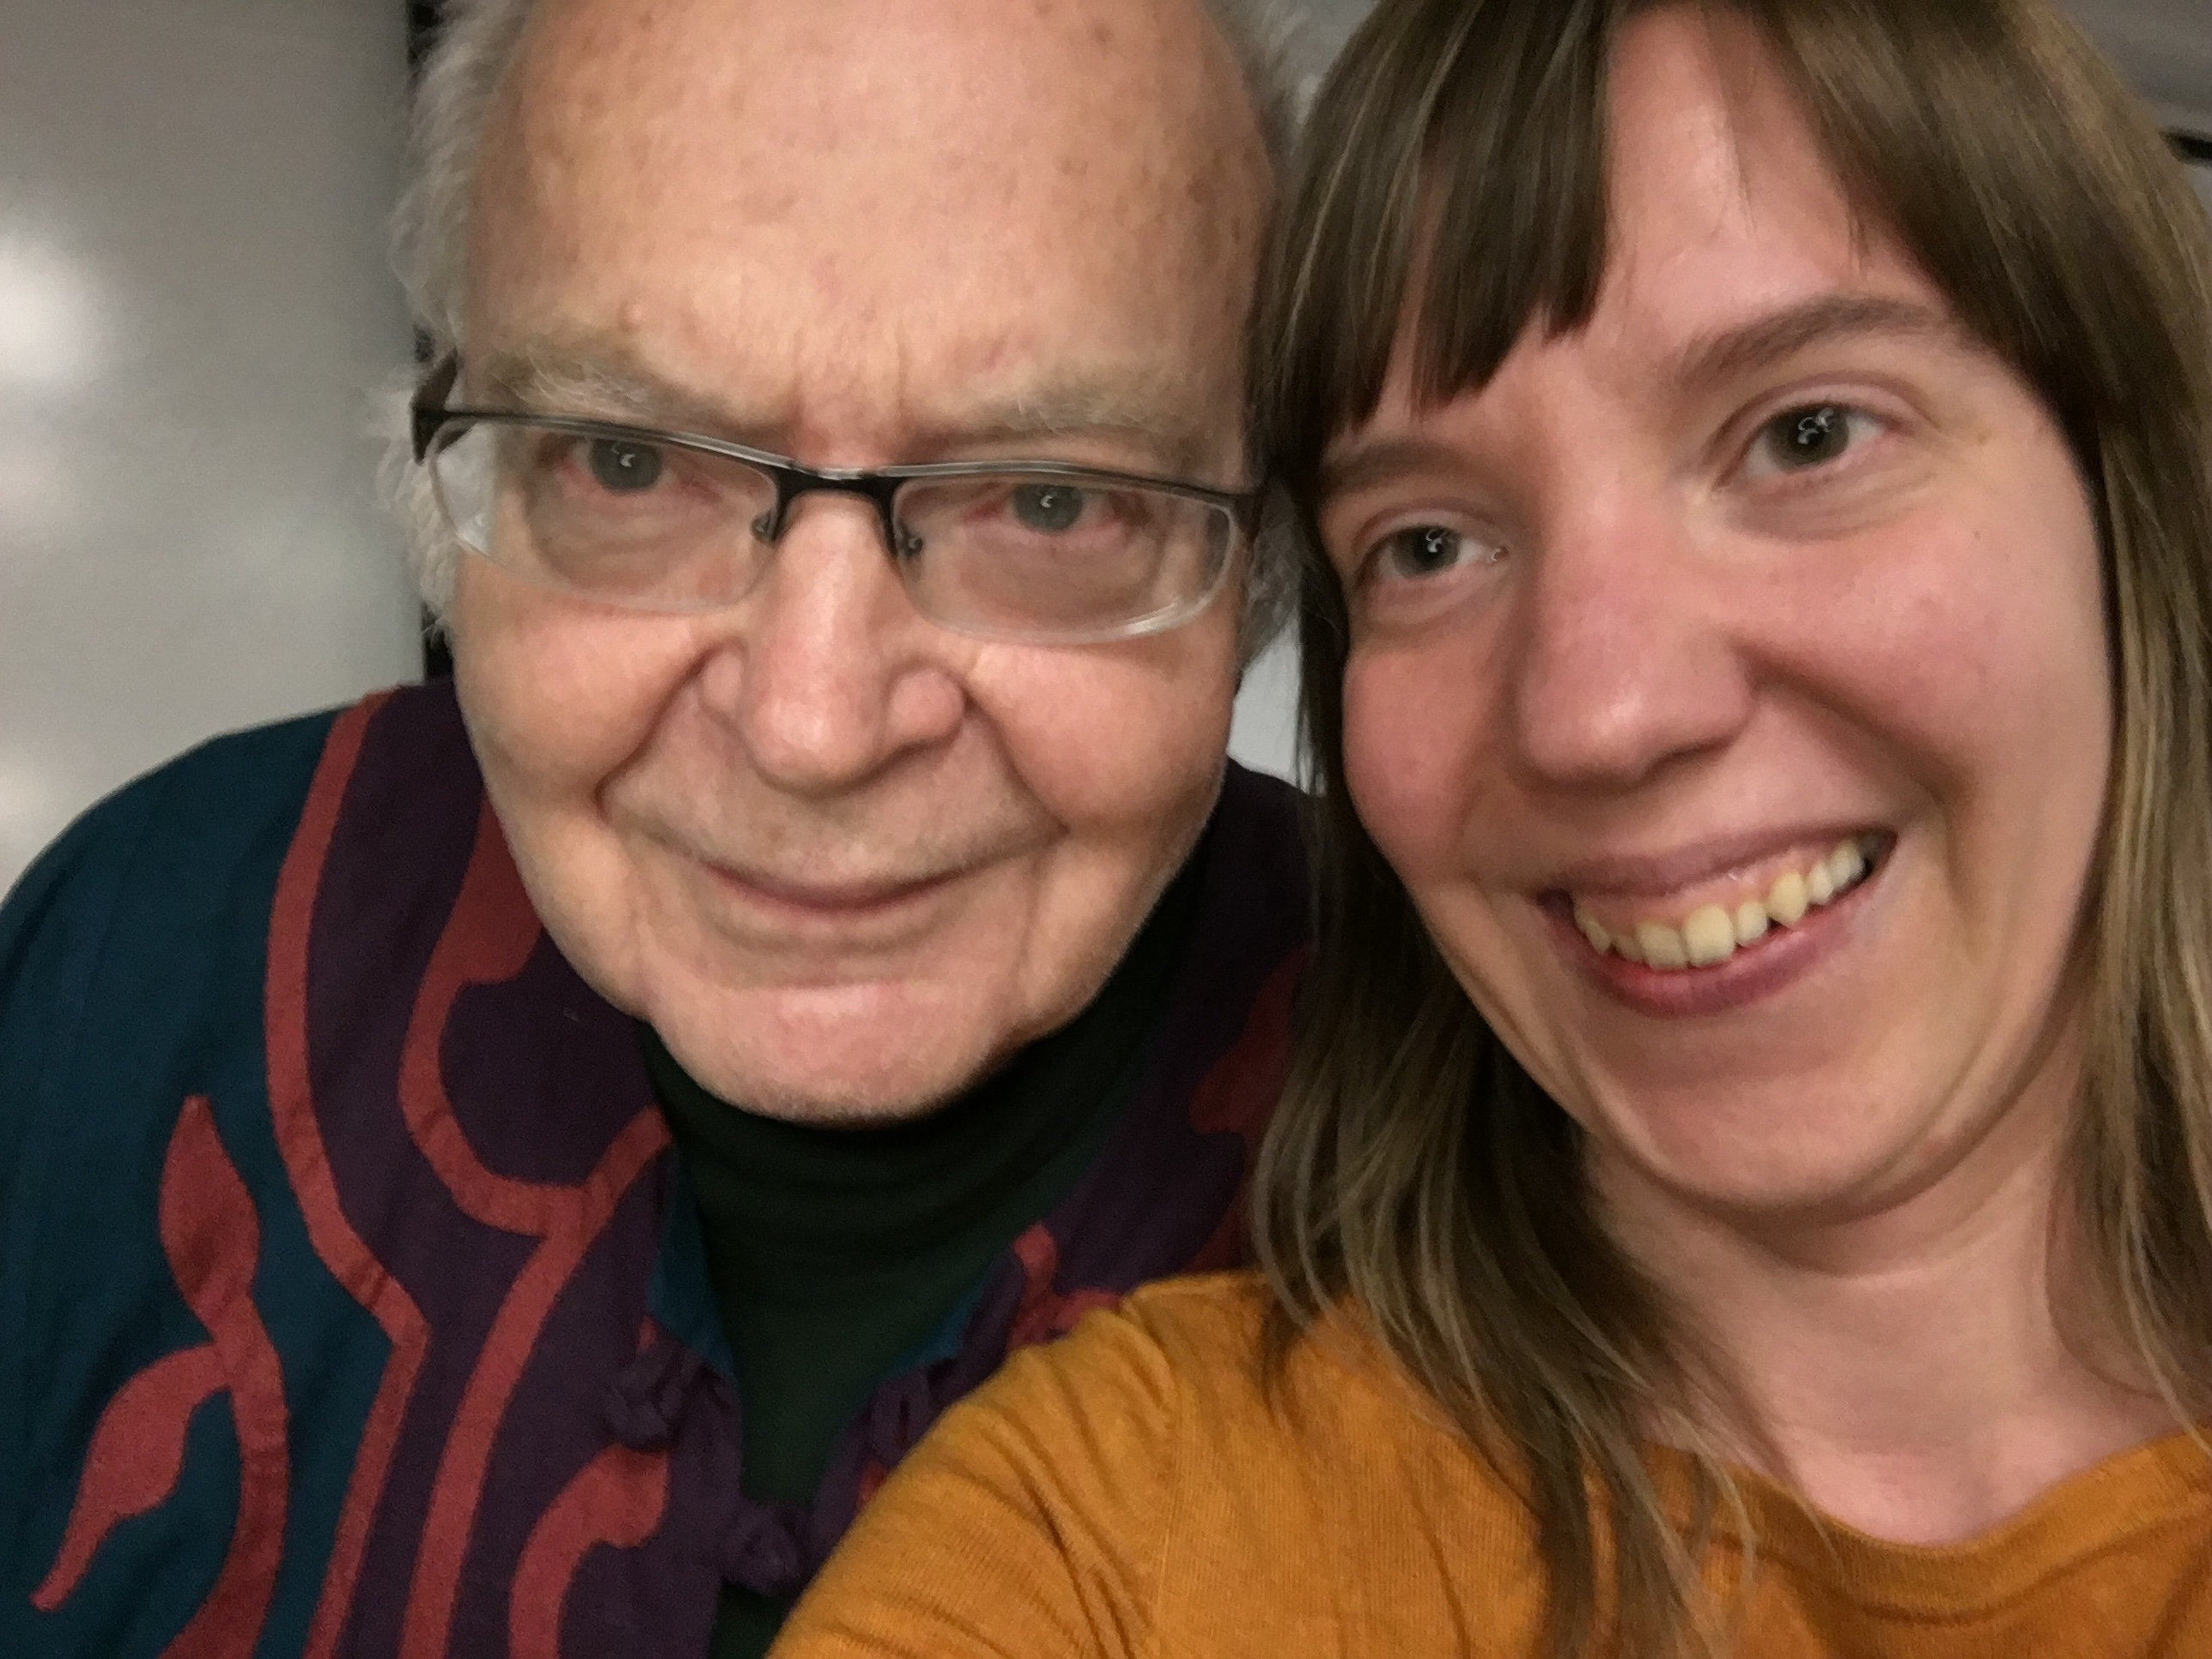
\includegraphics[width=\paperwidth,trim=0 483 0 0,clip]{knuth-katja.jpg}%
}
\begin{frame}
\end{frame}
\usebackgroundtemplate{}

\usebackgroundtemplate{%
  \makebox[\paperwidth]{
\includegraphics[height=\paperheight]{taocp.jpg}}%
}
\begin{frame}
\end{frame}
\usebackgroundtemplate{}

\begin{frame}
  \vspace{1em}
  \begin{center}
    {\Huge
      \begin{itemize}
        \item Vol.~1 (1968)
        \item Vol.~2 (1969)
        \item Vol.~3 (1973)
        \item<2> Vol.~2, druga izdaja (1976--1981)
        \item Vol.~4A (2011)
        \item Vol.~4B (2022)
      \end{itemize}
    }
  \end{center}
\end{frame}

% Knuth, Mathematical Typography, Bull. AMS 1 (1979), slika 1 (c), (i) in (k)
\begin{frame}{Transactions of the American Mathematical Society}
  \centering
  \only<1>{%
    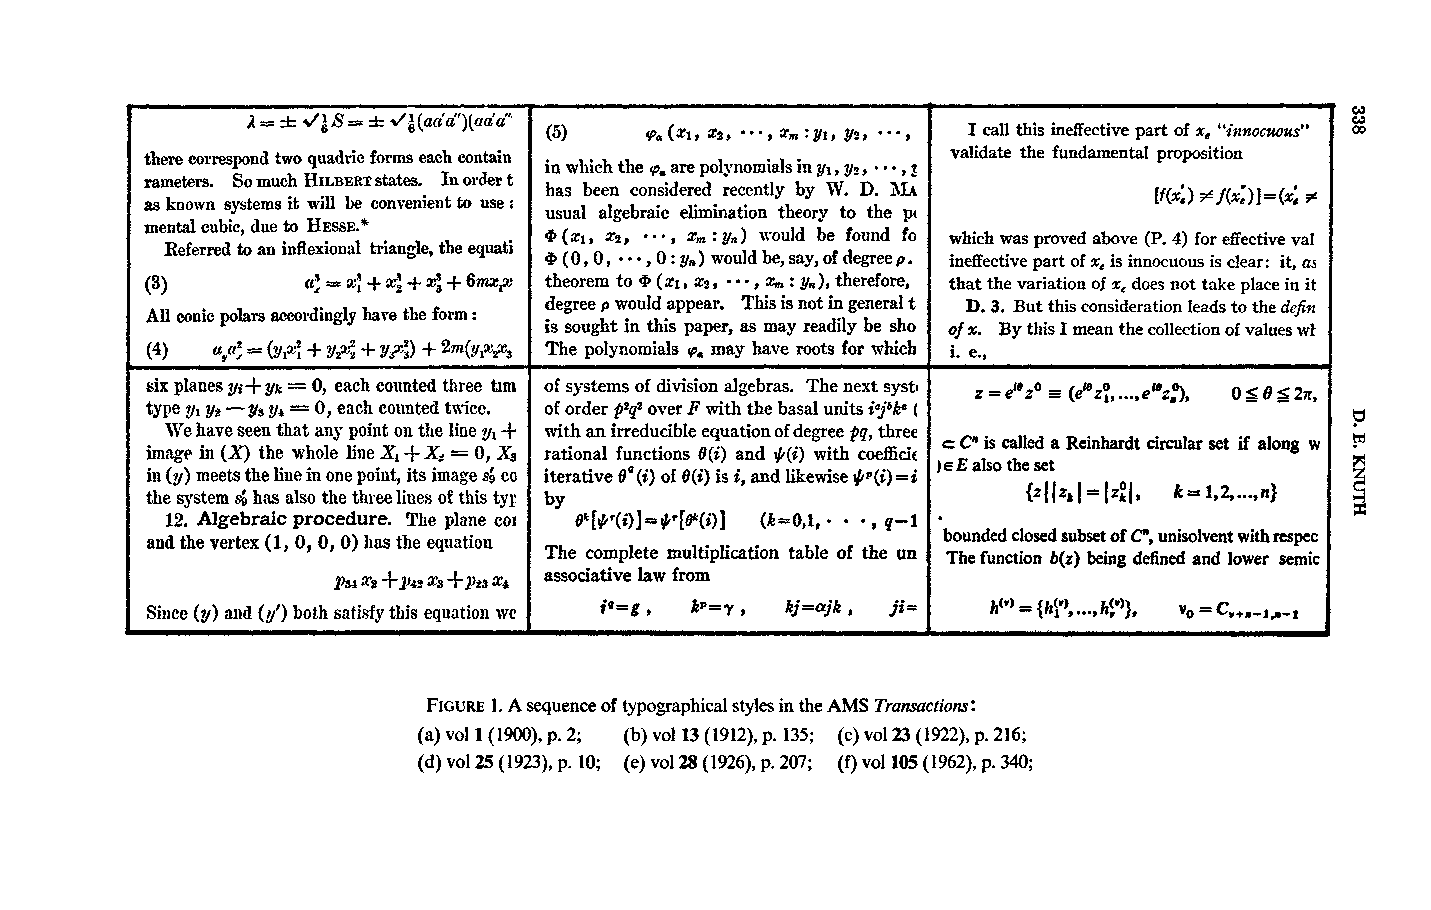
\includegraphics[height=0.6\textheight,page=1,trim=445 265 46 49,clip]{transactions-ams.pdf}\\[1ex]
    zvezek 23 (1922)%
  }%
  \only<2>{%
    \includegraphics[height=0.6\textheight,page=2,trim=445 268 46 49,clip]{transactions-ams.pdf}\\[1ex]
    zvezek 169 (1972)%
  }%
  \only<3>{%
    \includegraphics[height=0.6\textheight,page=2,trim=253 133 242 169,clip]{transactions-ams.pdf}\\[1ex]
    zvezek 199 (1974)%
  }
  \vfill
  {\scriptsize D.~E. Knuth, \emph{Mathematical Typography}, Bull.\ AMS 1 (1979), 337--372}
\end{frame}

\begin{frame}
  \vspace{1em}
  \begin{center}
    {\Huge \TeX\ (1978)}
  \end{center}
\end{frame}

\begin{frame}
  \vspace{1em}
  \begin{center}
    {\Huge Leslie Lamport}
    \bigskip

    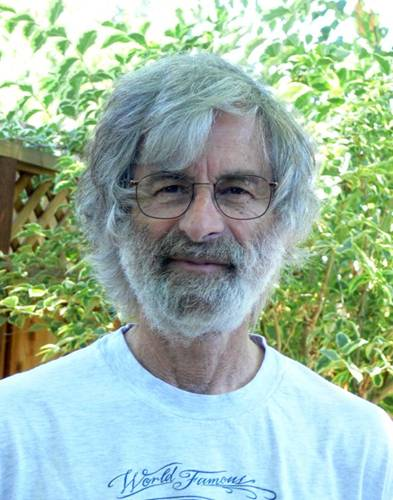
\includegraphics[height=0.65\textheight,keepaspectratio]{lamport.jpg}
    \smallskip

    dobitnik Turingove nagrade (2013)
  \end{center}
\end{frame}

\begin{frame}
  \vspace{1em}
  \begin{center}
    {\Huge \LaTeX\ (1984)}
  \end{center}
\end{frame}

\begin{frame}
  \vspace{1em}
  \begin{center}
    {\Huge 2026?}
  \end{center}
\end{frame}

\begin{frame}[fragile]{Markdown}

\begin{minted}{markdown}
# Naslov

Besedilo je lahko **poudarjeno** ter
vsebuje [povezave](https://www.fmf.uni-lj.si/),
`programsko kodo` in sezname:
- prva točka
- druga točka
- tretja točka
\end{minted}

\end{frame}

\begin{frame}[fragile]{HTML}

\begin{minted}{html}
<h1>Naslov</h1>

<p>Besedilo je lahko <strong>poudarjeno</strong> ter
vsebuje <a href="https://www.fmf.uni-lj.si/">povezave</a>,
<code>programsko kodo</code> in sezname:</p>
<ul>
  <li>prva točka</li>
  <li>druga točka</li>
  <li>tretja točka</li>
</ul>
\end{minted}

\end{frame}

\begin{frame}[fragile]{\LaTeX}

\begin{minted}{latex}
\section{Naslov}

Besedilo je lahko \textbf{poudarjeno} ter
vsebuje \href{https://www.fmf.uni-lj.si/}{povezave},
\texttt{programsko kodo} in sezname:

\begin{itemize}
  \item prva točka
  \item druga točka
  \item tretja točka
\end{itemize}
\end{minted}

\end{frame}

\begin{frame}[fragile]{Ukazi in okolja}

  \begin{block}{Ukazi}
    \begin{itemize}
      \item \mintinline{latex}|\ukaz|
      \item \mintinline{latex}|\ukaz{argument}|
      \item \mintinline{latex}|\ukaz[neobvezen]{argument}|
      \item \mintinline{latex}|\ukaz[neobvezen]{argument1}{argument2}|
    \end{itemize}
  \end{block}

  \begin{block}{Okolja}
    \begin{minted}{latex}
  \begin{okolje}
    ...
  \end{okolje}
    \end{minted}
  \end{block}
\end{frame}

\begin{frame}[fragile]{Nove odstavke naredimo s prazno vrstico}
  \begin{slaboenv}
    \begin{minted}[fontsize=\footnotesize]{latex}
Lorem ipsum dolor sit amet, consectetur adipiscing elit.
Ut id viverra ligula. Phasellus vehicula lorem vitae luctus
dignissim.
Sed ac justo commodo, fringilla urna ac, efficitur leo.
Praesent dui odio, accumsan ac sapien nec, interdum volutpat
est.
    \end{minted}

    Lorem ipsum dolor sit amet, consectetur adipiscing elit.
    Ut id viverra ligula. Phasellus vehicula lorem vitae luctus
    dignissim.
    Sed ac justo commodo, fringilla urna ac, efficitur leo.
    Praesent dui odio, accumsan ac sapien nec, interdum volutpat
    est.
  \end{slaboenv}
\end{frame}

\begin{frame}[fragile]{Nove odstavke naredimo s prazno vrstico}
  \begin{dobroenv}
    \begin{minted}[fontsize=\footnotesize]{latex}
Lorem ipsum dolor sit amet, consectetur adipiscing elit.
Ut id viverra ligula. Phasellus vehicula lorem vitae luctus
dignissim.

Sed ac justo commodo, fringilla urna ac, efficitur leo.
Praesent dui odio, accumsan ac sapien nec, interdum volutpat
est.
    \end{minted}

    Lorem ipsum dolor sit amet, consectetur adipiscing elit.
    Ut id viverra ligula. Phasellus vehicula lorem vitae luctus
    dignissim.

    Sed ac justo commodo, fringilla urna ac, efficitur leo.
    Praesent dui odio, accumsan ac sapien nec, interdum volutpat
    est.
  \end{dobroenv}
\end{frame}

\begin{frame}[fragile]{Nove odstavke naredimo s prazno vrstico}
  \begin{slaboenv}
    \begin{minted}[fontsize=\footnotesize]{latex}
Lorem ipsum dolor sit amet, consectetur adipiscing elit.
Ut id viverra ligula. Phasellus vehicula lorem vitae luctus
dignissim. \\
Sed ac justo commodo, fringilla urna ac, efficitur leo.
Praesent dui odio, accumsan ac sapien nec, interdum volutpat
est.
    \end{minted}

    Lorem ipsum dolor sit amet, consectetur adipiscing elit.
    Ut id viverra ligula. Phasellus vehicula lorem vitae luctus
    dignissim. \\
    Sed ac justo commodo, fringilla urna ac, efficitur leo.
    Praesent dui odio, accumsan ac sapien nec, interdum volutpat
    est.
  \end{slaboenv}
\end{frame}

\begin{frame}[fragile]{Matematika}
  \centering

  $$e^{i \pi} + 1 = 0$$
  \mintinline{latex}|e^{i \pi} + 1 = 0|

  $$\lim_{x \to 0} \frac{\sin x}{x} = 1$$
  \mintinline{latex}|\lim_{x \to 0} \frac{\sin x}{x} = 1|

  $$\int_{-\infty}^\infty e^{-x^2} \, dx = \sqrt{\pi}$$
  \mintinline{latex}|\int_{-\infty}^\infty e^{-x^2}\,dx = \sqrt{\pi}|

\end{frame}

\begin{frame}[fragile]{Vrstični in prikazni način}
  Naj bodo \(a, b, c \in \mathbb{R}\). Tedaj je
  \[
    x_{1, 2} = \frac{-b \pm \sqrt{b^2 - 4ac}}{2a}
  \]
  rešitev enačbe \(ax^2 + bx + c = 0\).

  \begin{minted}{latex}
Naj bodo \(a, b, c \in \mathbb{R}\). Tedaj je
\[
  x_{1, 2} = \frac{-b \pm \sqrt{b^2 - 4ac}}{2a}
\]
rešitev enačbe \(ax^2 + bx + c = 0\).
  \end{minted}
\end{frame}

\begin{frame}[fragile]{Vrstični in prikazni način}
  Naj bodo $a, b, c \in \mathbb{R}$. Tedaj je
  $$
  x_{1, 2} = \frac{-b \pm \sqrt{b^2 - 4ac}}{2a}
  $$
  rešitev enačbe $ax^2 + bx + c = 0$.

  \begin{minted}{latex}
Naj bodo $a, b, c \in \mathbb{R}$. Tedaj je
$$
  x_{1, 2} = \frac{-b \pm \sqrt{b^2 - 4ac}}{2a}
$$
rešitev enačbe $ax^2 + bx + c = 0$.
  \end{minted}
\end{frame}

\begin{frame}[fragile]{Vrstični in prikazni način}
  Naj bodo $a, b, c \in \mathbb{R}$. Tedaj je
  \[
    x_{1, 2} = \frac{-b \pm \sqrt{b^2 - 4ac}}{2a}
  \]
  rešitev enačbe $ax^2 + bx + c = 0$.

  \begin{minted}{latex}
Naj bodo $a, b, c \in \mathbb{R}$. Tedaj je
\[
  x_{1, 2} = \frac{-b \pm \sqrt{b^2 - 4ac}}{2a}
\]
rešitev enačbe $ax^2 + bx + c = 0$.
  \end{minted}
\end{frame}

\begin{frame}[fragile]{Uporabiti morate ustrezne ukaze}
  \begin{columns}[t]
    \begin{column}{0.45\textwidth}
      \begin{slaboenv}
        \begin{minted}{latex}
x \epsilon \mathbb{R}
        \end{minted}
        \[ x \epsilon \mathbb{R} \]
      \end{slaboenv}
    \end{column}
    \begin{column}{0.45\textwidth}
      \begin{dobroenv}
        \begin{minted}{latex}
x \in \mathbb{R}
        \end{minted}
        \[ x \in \mathbb{R} \]
      \end{dobroenv}
    \end{column}
  \end{columns}
\end{frame}

\begin{frame}[fragile]{Uporabiti morate ustrezne ukaze}
  \begin{columns}[t]
    \begin{column}{0.45\textwidth}
      \begin{slaboenv}
        \begin{minted}{latex}
\Sigma_{i=1}^n a_i^2 = 42
        \end{minted}
        \[ \Sigma_{i=1}^n a_i^2 = 42 \]
      \end{slaboenv}
    \end{column}
    \begin{column}{0.45\textwidth}
      \begin{dobroenv}
        \begin{minted}{latex}
\sum_{i=1}^n a_i^2 = 42
        \end{minted}
        \[ \sum_{i=1}^n a_i^2 = 42 \]
      \end{dobroenv}
    \end{column}
  \end{columns}
\end{frame}

\begin{frame}[fragile]{Uporabiti morate ustrezne ukaze}
  \begin{columns}[t]
    \begin{column}{0.45\textwidth}
      \begin{slaboenv}
        \begin{minted}{latex}
A \cap B = \phi
        \end{minted}
        \[ A \cap B = \phi \]
      \end{slaboenv}
    \end{column}
    \begin{column}{0.45\textwidth}
      \begin{dobroenv}
        \begin{minted}{latex}
A \cap B = \emptyset
        \end{minted}
        \[ A \cap B = \emptyset \]
      \end{dobroenv}
    \end{column}
  \end{columns}
\end{frame}

\begin{frame}[fragile]{Uporabiti morate ustrezne ukaze}
  \begin{columns}[t]
    \begin{column}{0.45\textwidth}
      \begin{slaboenv}
        \begin{minted}{latex}
2 <x, y> + 3 <y, x>
        \end{minted}
        \[ 2 <x, y> + 3 <y, x> \]
      \end{slaboenv}
    \end{column}
    \begin{column}{0.45\textwidth}
      \begin{dobroenv}
        \begin{minted}{latex}
2 \langle x, y \rangle
+ 3 \langle y, x \rangle
        \end{minted}
        \[ 2 \langle x, y \rangle + 3 \langle y, x \rangle \]
      \end{dobroenv}
    \end{column}
  \end{columns}
\end{frame}

\begin{frame}[fragile]{Za matematične operacije uporabimo ustrezne ukaze}
  \begin{columns}[t]
    \begin{column}{0.45\textwidth}
      \begin{slaboenv}
        \begin{minted}{latex}
sin x + sin (x + y)
        \end{minted}
        \[ sin x + sin (x + y) \]
      \end{slaboenv}
      \begin{slaboenv}
        \begin{minted}{latex}
sin~x + sin~(x + y)
        \end{minted}
        \[ sin~x + sin~(x + y) \]
      \end{slaboenv}
    \end{column}
    \begin{column}{0.45\textwidth}
      \begin{slaboenv}
        \begin{minted}[fontsize=\footnotesize]{latex}
\mathsf{sin}~x + \mathsf{sin}~(x + y)
        \end{minted}
        \[ \mathsf{sin}~x + \mathsf{sin}~(x + y) \]
      \end{slaboenv}
      \begin{dobroenv}
        \begin{minted}{latex}
\sin x + \sin (x + y)
        \end{minted}
        \[ \sin x + \sin (x + y) \]
      \end{dobroenv}
    \end{column}
  \end{columns}
\end{frame}

\begin{frame}[fragile]{Za sredinsko poravnane izraze uporabljamo prikazni način}
  \begin{columns}[t]
    \begin{column}{0.45\textwidth}
      \begin{slaboenv}
        \begin{minted}{latex}
\begin{center}
  \( e^{i \pi} + 1 = 0 \)
\end{center}
        \end{minted}
        \begin{center}
          \( e^{i \pi} + 1 = 0 \)
        \end{center}
      \end{slaboenv}
    \end{column}
    \begin{column}{0.45\textwidth}
      \begin{dobroenv}
        \begin{minted}{latex}
\[
  e^{i \pi} + 1 = 0
\]
        \end{minted}
        \[ e^{i \pi} + 1 = 0 \]
      \end{dobroenv}
    \end{column}
  \end{columns}
\end{frame}

\begin{frame}[fragile]{Za sredinsko poravnane izraze uporabljamo prikazni način}
  \begin{columns}[t]
    \begin{column}{0.45\textwidth}
      \begin{slaboenv}
        \begin{minted}[fontsize=\footnotesize]{latex}
\begin{center}
  \( x_{1, 2} = … \)
\end{center}
        \end{minted}
        \begin{center}
          \( x_{1, 2} = \frac{-b \pm \sqrt{b^2 - 4ac}}{2a} \)
        \end{center}
      \end{slaboenv}
    \end{column}
    \begin{column}{0.45\textwidth}
      \begin{dobroenv}
        \begin{minted}[fontsize=\footnotesize]{latex}
\[
  x_{1, 2} = …
\]
        \end{minted}
        \[ x_{1, 2} = \frac{-b \pm \sqrt{b^2 - 4ac}}{2a} \]
      \end{dobroenv}
    \end{column}
  \end{columns}
\end{frame}

\begin{frame}[fragile]{Struktura dokumenta}

\begin{minted}[fontsize=\footnotesize]{latex}
\documentclass[11pt,a4paper]{article}
% preambula
\usepackage[utf8]{inputenc}
\usepackage[T1]{fontenc}
\usepackage[slovene]{babel}

\title{Naslov dokumenta}
\author{Avtor dokumenta}
\date{\today}

\begin{document}
\maketitle
...vsebina...
\end{document}
\end{minted}
\end{frame}

\begin{frame}[fragile]{Ne vklapljajte nepotrebnih paketov}
  \begin{columns}[t]
    \begin{column}{0.45\textwidth}
      \begin{dobroenv}
        \begin{minted}[fontsize=\tiny]{latex}
\documentclass[11pt]{article}

\usepackage[utf8]{inputenc}
\usepackage[T1]{fontenc}

\usepackage[slovene]{babel}
\usepackage{lmodern}
\usepackage{amsmath}
\usepackage{amsfonts}
\usepackage{amsthm}
\usepackage{mathtools}
        \end{minted}
      \end{dobroenv}
    \end{column}
    \begin{column}{0.45\textwidth}
      \begin{slaboenv}
        \begin{minted}[fontsize=\tiny]{latex}
\documentclass[11pt]{article}

\usepackage[utf8]{inputenc}
% Ostale možnosti za kodiranje so:
% Kodirna tabela za Windows
% \usepackage[cp1250]{inputenc}
% Kodirna tabela za Linux
% \usepackage[latin2]{inputenc}
\usepackage[T1]{fontenc}

\usepackage[slovene]{babel}
\usepackage{lmodern}
\usepackage{amsmath}
\usepackage{amsfonts}
\usepackage{amsthm}
\usepackage{mathtools}
\usepackage{graphicx}
% \usepackage{tikz}
        \end{minted}
      \end{slaboenv}
    \end{column}
  \end{columns}
\end{frame}

\begin{frame}[fragile]{Pomožne datoteke}
  \begin{minted}{text}
dokument.aux
dokument.fdb_latexmk
dokument.fls
dokument.log
dokument.pdf
dokument.synctex.gz
dokument.tex
  \end{minted}
\end{frame}

\begin{frame}[fragile]{\texttt{.gitignore}}
  \begin{minted}{text}
*.aux
*.fdb_latexmk
*.fls
*.log
*.synctex.gz
*.pdf
  \end{minted}
  \bigskip

  Datoteka \texttt{.gitignore} velja samo za datoteke, ki jim Git še ne sledi.
\end{frame}

\begin{frame}[fragile]
  \begin{center}
    \Huge \LaTeX\ izven \LaTeX a
  \end{center}
\end{frame}

\end{document}
